\documentclass[a4paper]{article}
\usepackage{amsmath}
\usepackage{subfigure}
\usepackage{graphicx}
\usepackage{epstopdf}
\usepackage{caption}
\usepackage{multirow}
\usepackage{bigstrut}
\usepackage[top=2cm]{geometry}
\begin{document}
\title{CSE803: Homework\#2}
\author{Yuan Liang\\liangy11@msu.edu}
\date{}
\maketitle
\numberwithin{equation}{section}
\numberwithin{figure}{section}
\numberwithin{table}{section}
\section{Problem 1}
The program is written in Matlab. So the coordinate is row and column and the top left pixel of image is located at (1,1). The program contains serveral functions. Among them, function `img\_proc' is the integrated one that implements all the functionalities. The `img\_proc' has four input parameters: the path of the image file, format, threshold, and above\_below which indicates foreground should be greater (above\_below is greater than or equal to 0) or less than (otherwise) the threshold. The outputs of `img\_proc' includes the area, centroid, moments, inertia, circularity, circumference of each connected object in the image. Other functions in the program includes `raster\_scan\_8' which searches the connected componenents by using raster scan algorithm for 8 connected neighbor, `pepper\_salt' which cleans the pepper and salt noise in the image, `moments' which calculates the centroid and three moments of each object, `inertia' calculates the maximal and minimal inertia and the corresponding radians (the radian of the inertia axis from the horizontal line in clockwise), `dilate' which dilates object, `circularity' calculating the circularity of object and `circumference' which calculates the circumference of object by distracting the original image from the dilated image to get the boundary pixels.

For image `hw2-2B', the threshold I choose is 55, and foreground is greater than threshold. For image `hw2-3A' and `my', the threshold is 135 and foreground is less than threshold.

A sample command is
\begin{center}
	img\_proc(`hw2-3A',`jpg',135,-1)
\end{center}
Then it will print out the result in the command window of Matlab.

For image `hw2-2B', the original image and the image after thresholding are shown in figure \ref{figure:Hw2-2B image}, and the connected component analysis results are shown in table \ref{table:Hw2-2B analysis}. For the result of connected component recognition, see Problem 2. 
\begin{figure}[h]
	\begin{minipage}[c]{0.5\linewidth}
		% Requires \usepackage{graphicx}
		\centering
		\includegraphics{program/1/figure/Hw2-2B.eps}
		\caption*{(a) The original image}
		\label{subfigure:Hw2-2B-original}
	\end{minipage}
	\begin{minipage}[c]{0.5\linewidth}
		\centering
		\includegraphics{program/1/figure/Hw2-2B-threshold.eps}
		\caption*{(b) The image after thresholding}
		\label{subfigure:Hw2-2B-threshold}
	\end{minipage}
	\caption{Image of Hw2-2B}\label{figure:Hw2-2B image}
\end{figure}

For image `hw2-3A', the original image and the image after thresholding are shown in figure \ref{figure:Hw2-3A image}, and the connected component analysis results are shown in table \ref{table:Hw2-3A analysis}. There are 20 objects. Since the objects in the image are squares and rectangles, the rc moment should be close to zero because of symmetry, which is in accordance with the analysis results.   
\begin{figure}[h]
	\begin{minipage}[h]{0.5\linewidth}
		% Requires \usepackage{graphicx}
		\centering
		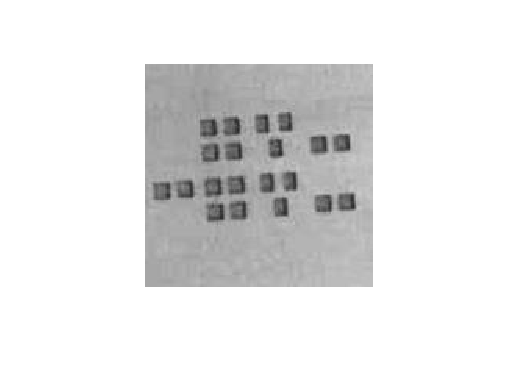
\includegraphics{program/1/figure/Hw2-3A.eps}
		\caption*{(a) The original image}
		\label{subfigure:Hw2-3A-original}
	\end{minipage}
	\begin{minipage}[h]{0.5\linewidth}
		\centering
		\includegraphics{program/1/figure/Hw2-3A-threshold.eps}
		\caption*{(b) The image after thresholding}
		\label{subfigure:Hw2-3A-threshold}
	\end{minipage}
	\caption{Image of Hw2-3A}\label{figure:Hw2-3A image}
\end{figure}

For the image `my.jpg' I took, the original image and the image after thresholding are shown in figure \ref{figure:my image}, and the connected component analysis results are shown in table \ref{table:my analysis}. Since the 3 objects in this image are circles, we can see from the analysis results that the rr and cc are large and similar while rc is close to 0, and that the maximal and minimal inertias are also close, and that the cirularity is large.
\begin{figure}[h]
	\begin{minipage}[h]{0.5\linewidth}
		% Requires \usepackage{graphicx}
		\centering
		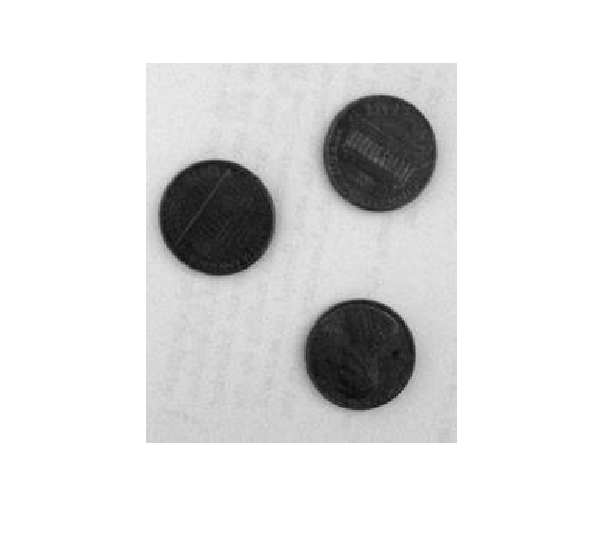
\includegraphics{program/1/figure/my.eps}
		\caption*{(a) The original image}
		\label{subfigure:my-original}
	\end{minipage}
	\begin{minipage}[h]{0.5\linewidth}
		\centering
		\includegraphics{program/1/figure/my-threshold.eps}
		\caption*{(b) The image after thresholding}
		\label{subfigure:my-threshold}
	\end{minipage}
	\caption{Image of `my.jpg'}\label{figure:my image}
\end{figure}

% Table generated by Excel2LaTeX from sheet 'Sheet1'
\newgeometry{left=0.2cm}
\begin{table}[p]
	\centering
	\caption{Connected component analysis of `Hw2-2B'}
	\begin{tabular}{|c|c|c|c|c|c|c|c|c|c|c|c|c|}
		\hline
		\multirow{2}[4]{*}{Region} & \multirow{2}[4]{*}{Area} & \multicolumn{2}{c|}{Centroid} & \multicolumn{3}{c|}{Moments} & \multicolumn{4}{c|}{Inertia}  & \multirow{2}[4]{*}{Circularity} & \multirow{2}[4]{*}{Perimeter} \bigstrut\\
		\cline{3-11}          &       & r     & c     & rr    & rc    & cc    & radian\_max & max   & radian\_min & min   &       &  \bigstrut\\
		\hline
		1     & 46    & 9.00  & 7.50  & 23.57  & 0.00  & 20.68  & 0.00  & 23.57  & 1.57  & 20.68  & 4.92  & 92 \bigstrut\\
		\hline
		2     & 12    & 6.50  & 5.00  & 1.25  & 0.00  & 0.67  & 0.00  & 1.25  & 1.57  & 0.67  & 6.71  & 18 \bigstrut\\
		\hline
		3     & 8     & 9.50  & 7.50  & 5.25  & -5.25  & 5.25  & 0.79  & 10.50  & 2.36  & 0.00  & 2.08  & 36 \bigstrut\\
		\hline
		4     & 11    & 18.00  & 7.00  & 0.00  & 0.00  & 10.00  & 1.57  & 10.00  & 0.00  & 0.00  & 2.08  & 28 \bigstrut\\
		\hline
	\end{tabular}%
	\label{table:Hw2-2B analysis}%
	
\end{table}%
\begin{table}[h]
	\centering
	\caption{Connected component analysis of `Hw2-3A'}
	\begin{tabular}{|c|c|c|c|c|c|c|c|c|c|c|c|c|}
		\hline
		\multirow{2}[4]{*}{Region} & \multirow{2}[4]{*}{Area} & \multicolumn{2}{c|}{Centroid} & \multicolumn{3}{c|}{Moments} & \multicolumn{4}{c|}{Inertia}  & \multirow{2}[4]{*}{Circularity} & \multirow{2}[4]{*}{Perimeter} \bigstrut\\
		\cline{3-11}          &       & r     & c     & rr    & rc    & cc    & radian\_max & max   & radian\_min & min   &       &  \bigstrut\\
		\hline
		1     & 107   & 38.96  & 75.88  & 12.30  & 0.63  & 6.33  & -0.10  & 12.36  & 1.47  & 6.27  & 6.96  & 53 \bigstrut\\
		\hline
		2     & 106   & 37.56  & 90.49  & 11.28  & 0.86  & 6.74  & -0.18  & 11.44  & 1.39  & 6.58  & 7.43  & 48 \bigstrut\\
		\hline
		3     & 127   & 40.50  & 56.13  & 11.43  & 0.02  & 9.48  & -0.01  & 11.43  & 1.56  & 9.48  & 9.51  & 54 \bigstrut\\
		\hline
		4     & 136   & 41.68  & 41.22  & 11.55  & 0.38  & 10.69  & -0.36  & 11.70  & 1.21  & 10.54  & 10.28  & 55 \bigstrut\\
		\hline
		5     & 109   & 51.12  & 126.62  & 9.70  & -0.23  & 8.29  & 0.16  & 9.74  & 1.73  & 8.25  & 9.16  & 48 \bigstrut\\
		\hline
		6     & 115   & 52.17  & 112.00  & 9.36  & -0.23  & 9.25  & 0.67  & 9.55  & 2.24  & 9.07  & 11.57  & 50 \bigstrut\\
		\hline
		7     & 101   & 54.41  & 84.54  & 11.51  & 1.01  & 6.15  & -0.18  & 11.69  & 1.39  & 5.97  & 6.58  & 48 \bigstrut\\
		\hline
		8     & 131   & 56.47  & 57.44  & 10.97  & 0.24  & 10.26  & -0.30  & 11.04  & 1.27  & 10.19  & 11.39  & 55 \bigstrut\\
		\hline
		9     & 137   & 57.45  & 42.71  & 11.60  & -0.28  & 10.76  & 0.29  & 11.69  & 1.86  & 10.68  & 10.79  & 56 \bigstrut\\
		\hline
		10    & 103   & 75.54  & 93.79  & 11.12  & 0.71  & 6.34  & -0.14  & 11.22  & 1.43  & 6.24  & 7.74  & 48 \bigstrut\\
		\hline
		11    & 106   & 76.49  & 79.05  & 11.68  & 0.15  & 6.35  & -0.03  & 11.69  & 1.54  & 6.34  & 7.50  & 48 \bigstrut\\
		\hline
		12    & 139   & 79.37  & 44.37  & 11.99  & -0.06  & 10.88  & 0.05  & 11.99  & 1.62  & 10.88  & 9.86  & 58 \bigstrut\\
		\hline
		13    & 130   & 78.21  & 59.08  & 10.49  & -0.15  & 10.92  & 1.26  & 10.97  & -0.31  & 10.44  & 10.01  & 57 \bigstrut\\
		\hline
		14    & 129   & 80.70  & 26.55  & 10.63  & 0.68  & 10.57  & -0.76  & 11.28  & 0.81  & 9.92  & 9.64  & 55 \bigstrut\\
		\hline
		15    & 125   & 81.87  & 11.70  & 10.11  & 0.30  & 10.70  & 1.96  & 10.83  & 0.39  & 9.99  & 8.73  & 54 \bigstrut\\
		\hline
		16    & 117   & 89.04  & 129.73  & 9.46  & 0.56  & 9.60  & 2.29  & 10.09  & 0.72  & 8.97  & 10.66  & 50 \bigstrut\\
		\hline
		17    & 117   & 90.00  & 115.00  & 9.49  & 0.00  & 9.49  & 0.79  & 9.49  & 0.79  & 9.49  & 10.97  & 48 \bigstrut\\
		\hline
		18    & 112   & 92.38  & 87.54  & 11.74  & 0.62  & 7.11  & -0.13  & 11.82  & 1.44  & 7.03  & 8.04  & 50 \bigstrut\\
		\hline
		19    & 130   & 95.26  & 45.76  & 11.45  & -0.07  & 10.04  & 0.05  & 11.46  & 1.62  & 10.04  & 9.37  & 54 \bigstrut\\
		\hline
		20    & 133   & 94.39  & 60.53  & 10.90  & 0.02  & 10.62  & -0.09  & 10.90  & 1.48  & 10.62  & 11.94  & 54 \bigstrut\\
		\hline
	\end{tabular}%
	\label{table:Hw2-3A analysis}%
\end{table}%

\begin{table}[h]
	\centering
	\caption{Connected component analysis of `my.jpg'}
	\begin{tabular}{|c|c|c|c|c|c|c|c|c|c|c|c|c|}
		\hline
		\multirow{2}[4]{*}{Region} & \multirow{2}[4]{*}{Area} & \multicolumn{2}{c|}{Centroid} & \multicolumn{3}{c|}{Moments} & \multicolumn{4}{c|}{Inertia}  & \multirow{2}[4]{*}{Circularity} & \multirow{2}[4]{*}{Perimeter} \bigstrut\\
		\cline{3-11}          &       & r     & c     & rr    & rc    & cc    & radian\_max & max   & radian\_min & min   &       &  \bigstrut\\
		\hline
		1     & 4395  & 58.39  & 151.04  & 359.53  & -4.88  & 340.32  & 0.24  & 360.70  & 1.81  & 339.15  & 67.20  & 304 \bigstrut\\
		\hline
		2     & 4458  & 99.95  & 46.54  & 352.29  & 10.99  & 357.59  & 2.24  & 366.25  & 0.67  & 343.63  & 66.65  & 306 \bigstrut\\
		\hline
		3     & 4082  & 188.03  & 138.29  & 323.83  & -0.61  & 325.87  & 1.30  & 326.04  & -0.27  & 323.66  & 93.48  & 295.41  \bigstrut\\
		\hline
	\end{tabular}%
	\label{table:my analysis}%
\end{table}%

\restoregeometry

\section{Problem 2}
The connected component recognition of `Hw2-2A' and `Hw2-2B' are shown in table \ref{table: Hw2-2A connected} and table \ref{table: Hw2-2B connected} respectively and the area and centroid of each region are listed in table \ref{table: Hw2-2A centroid} and table \ref{table: Hw2-2B centroid} respectively. We can easily see the corresponding reigons between the two images while their ordinals are permuted. The region 1 and 2 in `Hw2-2B' correspond to region 2 and 4 in `Hw2-2A'. By using their centroids, according to the equation (11.10) in textbook, the radian of rotation is $\frac{\pi}{2}$ clockwise and the translation is 21 pixels in column positively and 0 pixel in row. The centroid of each region after mapping `Hw2-2B' is shown in table \ref{table: centroid mapped}. We can see that even though the ordinals are permuted, the mapped positions are equal to those of the corresponding regions in `Hw2-2A', so the mapping error should be zero.

% Table generated by Excel2LaTeX from sheet 'Sheet1'
\begin{table}[h]
	\centering
	\caption{Connected component recognition of Hw2-2A}
	\begin{tabular}{|r|r|r|r|r|r|r|r|r|r|r|r|r|r|r|r|r|r|r|r|}
		\hline
		0     & 0     & 0     & 0     & 0     & 0     & 0     & 0     & 0     & 0     & 0     & 0     & 0     & 0     & 0     & 0     & 0     & 0     & 0     & 0 \bigstrut\\
		\hline
		0     & 0     & 1     & 0     & 0     & 2     & 2     & 2     & 2     & 2     & 2     & 2     & 2     & 2     & 2     & 2     & 2     & 2     & 0     & 0 \bigstrut\\
		\hline
		0     & 0     & 1     & 0     & 0     & 2     & 0     & 0     & 0     & 0     & 0     & 0     & 0     & 0     & 0     & 0     & 0     & 2     & 0     & 0 \bigstrut\\
		\hline
		0     & 0     & 1     & 0     & 0     & 2     & 0     & 3     & 0     & 0     & 0     & 0     & 4     & 4     & 4     & 4     & 0     & 2     & 0     & 0 \bigstrut\\
		\hline
		0     & 0     & 1     & 0     & 0     & 2     & 0     & 0     & 3     & 0     & 0     & 0     & 4     & 4     & 4     & 4     & 0     & 2     & 0     & 0 \bigstrut\\
		\hline
		0     & 0     & 1     & 0     & 0     & 2     & 0     & 0     & 0     & 3     & 0     & 0     & 4     & 4     & 4     & 4     & 0     & 2     & 0     & 0 \bigstrut\\
		\hline
		0     & 0     & 1     & 0     & 0     & 2     & 0     & 0     & 0     & 0     & 3     & 0     & 0     & 0     & 0     & 0     & 0     & 2     & 0     & 0 \bigstrut\\
		\hline
		0     & 0     & 1     & 0     & 0     & 2     & 0     & 0     & 0     & 0     & 0     & 3     & 0     & 0     & 0     & 0     & 0     & 2     & 0     & 0 \bigstrut\\
		\hline
		0     & 0     & 1     & 0     & 0     & 2     & 0     & 0     & 0     & 0     & 0     & 0     & 3     & 0     & 0     & 0     & 0     & 2     & 0     & 0 \bigstrut\\
		\hline
		0     & 0     & 1     & 0     & 0     & 2     & 0     & 0     & 0     & 0     & 0     & 0     & 0     & 3     & 0     & 0     & 0     & 2     & 0     & 0 \bigstrut\\
		\hline
		0     & 0     & 1     & 0     & 0     & 2     & 0     & 0     & 0     & 0     & 0     & 0     & 0     & 0     & 3     & 0     & 0     & 2     & 0     & 0 \bigstrut\\
		\hline
		0     & 0     & 1     & 0     & 0     & 2     & 0     & 0     & 0     & 0     & 0     & 0     & 0     & 0     & 0     & 0     & 0     & 2     & 0     & 0 \bigstrut\\
		\hline
		0     & 0     & 0     & 0     & 0     & 2     & 2     & 2     & 2     & 2     & 2     & 2     & 2     & 2     & 2     & 2     & 2     & 2     & 0     & 0 \bigstrut\\
		\hline
		0     & 0     & 0     & 0     & 0     & 0     & 0     & 0     & 0     & 0     & 0     & 0     & 0     & 0     & 0     & 0     & 0     & 0     & 0     & 0 \bigstrut\\
		\hline
		0     & 0     & 0     & 0     & 0     & 0     & 0     & 0     & 0     & 0     & 0     & 0     & 0     & 0     & 0     & 0     & 0     & 0     & 0     & 0 \bigstrut\\
		\hline
	\end{tabular}%
	\label{table: Hw2-2A connected}%
\end{table}%
% Table generated by Excel2LaTeX from sheet 'Sheet1'
\begin{table}[h]
	\centering
	\caption{Connected component recognition of Hw2-2B}
	\begin{tabular}{|r|r|r|r|r|r|r|r|r|r|r|r|r|r|r|}
		\hline
		0     & 0     & 0     & 0     & 0     & 0     & 0     & 0     & 0     & 0     & 0     & 0     & 0     & 0     & 0 \bigstrut\\
		\hline
		0     & 0     & 0     & 0     & 0     & 0     & 0     & 0     & 0     & 0     & 0     & 0     & 0     & 0     & 0 \bigstrut\\
		\hline
		0     & 1     & 1     & 1     & 1     & 1     & 1     & 1     & 1     & 1     & 1     & 1     & 1     & 0     & 0 \bigstrut\\
		\hline
		0     & 1     & 0     & 0     & 0     & 0     & 0     & 0     & 0     & 0     & 0     & 0     & 1     & 0     & 0 \bigstrut\\
		\hline
		0     & 1     & 0     & 2     & 2     & 2     & 0     & 0     & 0     & 0     & 0     & 0     & 1     & 0     & 0 \bigstrut\\
		\hline
		0     & 1     & 0     & 2     & 2     & 2     & 0     & 0     & 0     & 0     & 3     & 0     & 1     & 0     & 0 \bigstrut\\
		\hline
		0     & 1     & 0     & 2     & 2     & 2     & 0     & 0     & 0     & 3     & 0     & 0     & 1     & 0     & 0 \bigstrut\\
		\hline
		0     & 1     & 0     & 2     & 2     & 2     & 0     & 0     & 3     & 0     & 0     & 0     & 1     & 0     & 0 \bigstrut\\
		\hline
		0     & 1     & 0     & 0     & 0     & 0     & 0     & 3     & 0     & 0     & 0     & 0     & 1     & 0     & 0 \bigstrut\\
		\hline
		0     & 1     & 0     & 0     & 0     & 0     & 3     & 0     & 0     & 0     & 0     & 0     & 1     & 0     & 0 \bigstrut\\
		\hline
		0     & 1     & 0     & 0     & 0     & 3     & 0     & 0     & 0     & 0     & 0     & 0     & 1     & 0     & 0 \bigstrut\\
		\hline
		0     & 1     & 0     & 0     & 3     & 0     & 0     & 0     & 0     & 0     & 0     & 0     & 1     & 0     & 0 \bigstrut\\
		\hline
		0     & 1     & 0     & 3     & 0     & 0     & 0     & 0     & 0     & 0     & 0     & 0     & 1     & 0     & 0 \bigstrut\\
		\hline
		0     & 1     & 0     & 0     & 0     & 0     & 0     & 0     & 0     & 0     & 0     & 0     & 1     & 0     & 0 \bigstrut\\
		\hline
		0     & 1     & 1     & 1     & 1     & 1     & 1     & 1     & 1     & 1     & 1     & 1     & 1     & 0     & 0 \bigstrut\\
		\hline
		0     & 0     & 0     & 0     & 0     & 0     & 0     & 0     & 0     & 0     & 0     & 0     & 0     & 0     & 0 \bigstrut\\
		\hline
		0     & 0     & 0     & 0     & 0     & 0     & 0     & 0     & 0     & 0     & 0     & 0     & 0     & 0     & 0 \bigstrut\\
		\hline
		0     & 4     & 4     & 4     & 4     & 4     & 4     & 4     & 4     & 4     & 4     & 4     & 0     & 0     & 0 \bigstrut\\
		\hline
		0     & 0     & 0     & 0     & 0     & 0     & 0     & 0     & 0     & 0     & 0     & 0     & 0     & 0     & 0 \bigstrut\\
		\hline
		0     & 0     & 0     & 0     & 0     & 0     & 0     & 0     & 0     & 0     & 0     & 0     & 0     & 0     & 0 \bigstrut\\
		\hline
	\end{tabular}%
	\label{table: Hw2-2B connected}%
\end{table}%

% Table generated by Excel2LaTeX from sheet 'Sheet1'
\begin{table}[h]
	\centering
	\caption{Area and centroid of each region in Hw2-2A}
	\begin{tabular}{|c|c|c|c|}
		\hline
		\multirow{2}[4]{*}{Region\#} & \multirow{2}[4]{*}{Area} & \multicolumn{2}{c|}{Centroid} \bigstrut\\
		\cline{3-4}          &       & r     & c \bigstrut\\
		\hline
		1     & 11    & 7     & 3 \bigstrut\\
		\hline
		2     & 46    & 7.5   & 12 \bigstrut\\
		\hline
		3     & 8     & 7.5   & 11.5 \bigstrut\\
		\hline
		4     & 12    & 5     & 14.5 \bigstrut\\
		\hline
	\end{tabular}%
	\label{table: Hw2-2A centroid}%
\end{table}%

\begin{table}[h]
	\centering
	\caption{Area and centroid of each region in Hw2-2B}
	\begin{tabular}{|c|c|c|c|}
		\hline
		\multirow{2}[4]{*}{Region\#} & \multirow{2}[4]{*}{Area} & \multicolumn{2}{c|}{Centroid} \bigstrut\\
		\cline{3-4}          &       & r     & c \bigstrut\\
			\hline
			1     & 46    & 9     & 7.5 \bigstrut\\
			\hline
			2     & 12    & 6.5   & 5 \bigstrut\\
			\hline
			3     & 8     & 9.5   & 7.5 \bigstrut\\
			\hline
			4     & 11    & 18    & 7 \bigstrut\\
			\hline
	\end{tabular}%
	\label{table: Hw2-2B centroid}%
\end{table}%

\begin{table}[h]
	\centering
	\caption{Centroid of each region by mapping Hw2-2B}
	\begin{tabular}{|c|c|c|}
		\hline
		\multirow{2}[4]{*}{Region\#} &  \multicolumn{2}{c|}{Centroid} \bigstrut\\
		\cline{2-3}            & r     & c \bigstrut\\
	 \hline
	 1     & 7.5 & 12 \bigstrut\\
	 \hline
	 2     & 5 & 14.5 \bigstrut\\
	 \hline
	 3     & 7.5 & 11.5 \bigstrut\\
	 \hline
	 4     & 7 & 3   \bigstrut\\
	 \hline
	 
	\end{tabular}%
	\label{table: centroid mapped}%
\end{table}%
\end{document} 